% This template was initially provided by Dulip Withanage.
% Modifications for the database systems research group
% were made by Conny Junghans,  Jannik Strötgen and Michael Gertz

\documentclass[
     12pt,         % font size
     a4paper,      % paper format
     BCOR10mm,     % binding correction
     DIV14,        % stripe size for margin calculation
     ]{article}

%%%%%%%%%%%%%%%%%%%%%%%%%%%%%%%%%%%%%%%%%%%%%%%%%%%%%%%%%%%%

% PACKAGES:

% Use German
\usepackage[english]{babel}
% Input and font encoding
\usepackage[latin1]{inputenc}
\usepackage[T1]{fontenc}
% Index-generation
\usepackage{makeidx}
% Embedding of URLs
\usepackage{url}
% Special \LaTex symbols (e.g. \BibTeX)
%\usepackage{doc}
% Include Graphic-files
\usepackage{graphicx}
% Include doc++ generated tex-files
%\usepackage{docxx}
% Fuer anderthalbzeiligen Textsatz
\usepackage{setspace}
\usepackage[table,xcdraw]{xcolor}
\usepackage{hhline}
\usepackage{highlight}

\usepackage{subcaption}

\usepackage{biblatex}
\bibliography{references.bib}

% hyperrefs in the documents
\PassOptionsToPackage{hyphens}{url}\usepackage[bookmarks=true,colorlinks,pdfpagelabels,pdfstartview = FitH,bookmarksopen = true,bookmarksnumbered = true,linkcolor = black,plainpages = false,hypertexnames = false,citecolor = black,urlcolor=black]{hyperref}
%\usepackage{hyperref}


% CUSTOM:

% For quotes:
\usepackage{csquotes}

% For Definitions:                   						
\usepackage{amsthm}
\usepackage[framemethod=tikz]{mdframed}
\usepackage{amsfonts}

\newtheoremstyle{defi}
{\topsep}         % Abstand oben
{\topsep}         % Abstand unten
{\normalfont}     % Schrift des Bodys
{0pt}             % Einschub der ersten Zeile
{\bfseries}       % Darstellung von der Schrift in der �berschrift
{:}               % Trennzeichen zwischen �berschrift und Body
{.5em}            % Abstand nach dem Trennzeichen zum Body Text
{\thmname{#3}}    % Name in eckigen Klammern
\theoremstyle{defi}

\newmdtheoremenv[
hidealllines = true,       % Rahmen komplett ausblenden
leftline = true,           % Linie links einschalten
innertopmargin = 0pt,      % Abstand oben
innerbottommargin = 4pt,   % Abstand unten
innerrightmargin = 0pt,    % Abstand rechts
linewidth = 3pt,           % Linienbreite
linecolor = gray!40,       % Linienfarbe
]{defStrich}{Definition}     % Name der des formats "defStrich"



%%%%%%%%%%%%%%%%%%%%%%%%%%%%%%%%%%%%%%%%%%%%%%%%%%%%%%%%%%%%

% OTHER SETTINGS:

% Choose language
\newcommand{\setlang}[1]{\selectlanguage{#1}\nonfrenchspacing}


\begin{document}

% TITLE:
\pagenumbering{roman} 
\begin{titlepage}

\vspace*{1cm}
\begin{center}
\textbf{ 
\Large Heidelberg University\\
\smallskip
\Large BioQuant, IPMB\\
\smallskip
\Large Biomedical Computer Vision Group (BMCV) \\
\smallskip
}

\vspace{3cm}

\textbf{\large Seminar Deep Learning for Biomedical Image Analysis}

Summer semester 2022

PD Dr. Karl Rohr

\vspace{1cm}
Mentor: Carola Krug



\vspace{3cm}

\textbf{\large Report for the seminar presentation}

\vspace{0.5\baselineskip}
{\LARGE\textbf{BrainGNN: Interpretable Brain Graph Neural Network for fMRI Analysis \cite{LI2021102233}}
}
\vspace{0.5cm}

%\url{https://github.com/fidsusj/HateSpeechDetection}


\end{center}

\vfill 

{\large
\begin{tabular}[l]{ll}
Student: & Nils Krehl, 3664130,\\
  & Data and Computer Science\\
  & nils.krehl@stud.uni-heidelberg.de\\
  
\end{tabular}
}

\end{titlepage}

\section*{Abstract}

The area of neuroscience deals with the understanding of the brain. Especially interesting is the connection of different brain regions to specific neurological disorders or cognitive stimuli. 
In the work by Li et al. \cite{LI2021102233} a novel Brain Graph Neural Network is proposed to analyze the data obtained through fMRI imaging of the brain. The novelties of this work are a new graph convolutional layer and the interpretability of the model results. 
The proposed model outperforms all compared baseline architectures in the prediction task on two evaluation datasets. Furthermore, the insights gained through the model's interpretability could be verified by literature.
%\section*{Plagiarism statement}

We certify that this report is our own work, based on our personal study and/or research and that we have acknowledged all material and sources used in its preparation, whether they be books, articles, reports, lecture notes, and any other kind of document, electronic or personal communication.
We also certify that this report has not previously been submitted for assessment in any other unit, except where specific permission has been granted from all unit coordinators involved, or at any other time in this unit, and that we have not copied in part or whole or otherwise plagiarized the work of other students and/or persons.


\newpage
\tableofcontents
\newpage

\pagenumbering{arabic}

\section{Introduction}

The area of modern neuroscience deals with the understanding of the brain. From special interest is the connection of specific parts of the brain to neurological disorders or cognitive stimuli. 
Based on this, patterns of specific neurological diseases can be detected and a personalized treatment for patients can be developed.

This report summarizes the work by Li et al. \cite{LI2021102233} about "BrainGNN: In\-ter\-pre\-ta\-ble Brain Graph Neural Network for fMRI Analysis".
The work by Li et al. is located in the area of modern neuroscience. 
Through fMRI (functional magnetic resonance imaging) the brain is observed. Based on these fMRI recordings, a graph of the brain is built. The nodes of the graph correspond to different brain regions and the edges describe interactions between different brain regions. This work then proposes a Brain Graph Neural Network (BrainGNN) for graph classification (e.g. is a person healthy or has a specific neurological disease?).
The main novelties proposed of this work are an improved graph convolutional layer and the inbuilt model interpretability.
\section{Related Work} \label{related_work}

The work by Li et al. \cite{LI2021102233} is the continuation of Li et al. \cite{10.1007/978-3-030-59728-3_61}. In addition to \cite{10.1007/978-3-030-59728-3_61} in \cite{LI2021102233} a new graph convolutional layer is proposed and a new dataset is used for evaluation.

In the recent past, Graph Neural Networks (GNN) have developed to the state-of-the-art method for graph based data science tasks.
A GNN uses a graph (with node features, edge features, graph topology) as input for a neural network. GNNs are a generalization of Convolutional Neural Networks (CNN).
The general applicability of GNNs was shown in various works, e.g. Kim and Ye \cite{10.3389/fnins.2020.00630},  Kazi et al. \cite{10.1007/978-3-030-20351-1_6}, Yan et al. \cite{10.1145/3292500.3330921}, Yang et al. \cite{10.1007/978-3-030-32248-9_89}, Gopinath et al. \cite{10.1007/978-3-030-20351-1_7} and Nandakumar et al. \cite{10.1007/978-3-030-32391-2_2}.

Depending on the application domain of the GNNs the underlying graphs have different properties. For example in social networks or protein networks the nodes of different instances are not related. Therefore, in this case the same embeddings are used for different nodes. 
Also for the analysis of fMRI images GNNs with the same embedding for different nodes are used. 
This assumes, that the different parts of the brain behave similar. This is not the case. That is why the work by Li et al. \cite{LI2021102233} models the brain with different embeddings for each node.

For the detection of biomarkers, there have been studies for group-level and individual-level biomarkers. Group-level biomarkers detect the common patterns of a specific disease and are explored by Li et al. \cite{10.1007/978-3-030-00931-1_24}, Venkataraman et al. \cite{Venkataraman2016BayesianCD}, Salman et al. \cite{SALMAN2019101747} and Yan et al. \cite{10.1145/3292500.3330921}. 
Individual-level biomarker are examined by Brennan et al. \cite{BRENNAN201927}, Mahowald and Fedorenko \cite{MAHOWALD201674} and Li et al. \cite{10.1007/978-3-030-32254-0_54}. These biomarkers are specific for one patient and are the basis for precision medicine. 
The work by Li et al. \cite{LI2021102233} investigates both, group-level and individual-level biomarkers.

Another modeling question is, what the nodes and the whole graph represent. In Parisot et al. \cite{PARISOT2018117} and Kazi et al. \cite{10.1007/978-3-030-20351-1_6} each patient is one node in the graph. The work by Li et al. \cite{LI2021102233} constructs one graph for the brain of each patient.

\section{Approach} 
\label{approach}

\subsection{Experiment pipeline}
\label{approach:A}

\begin{figure}[ht]
	\centering
	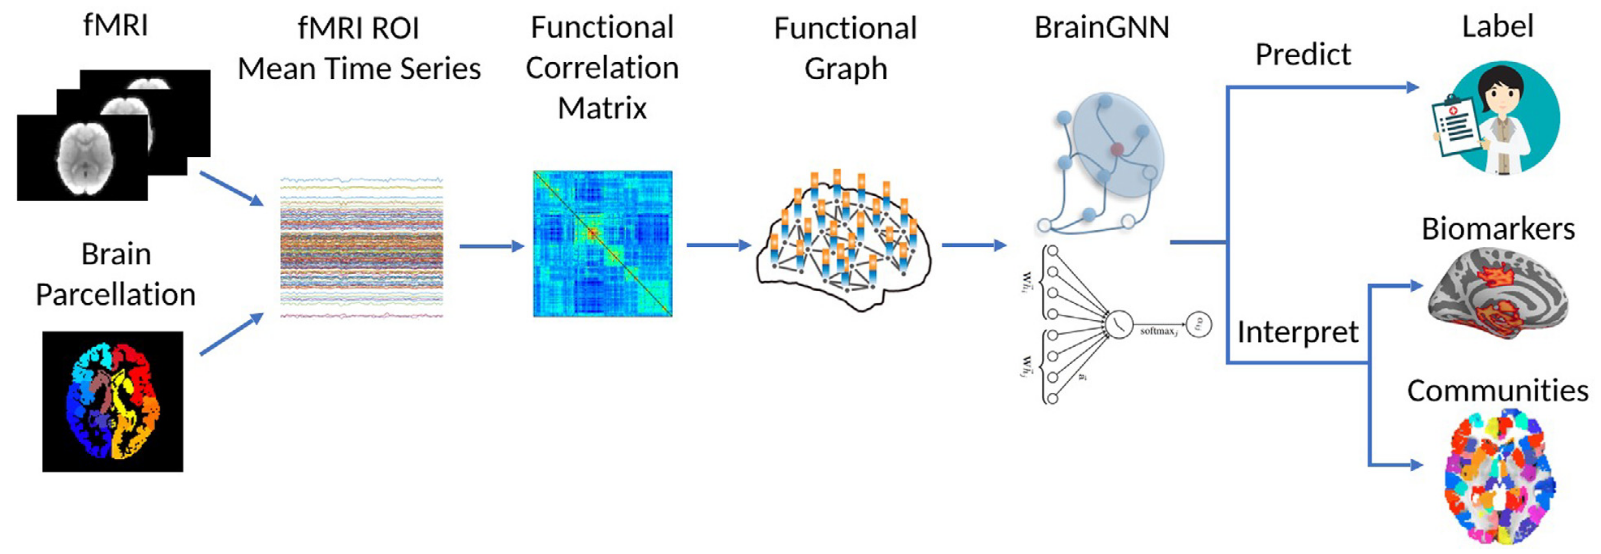
\includegraphics[width=1.0\linewidth]{figures/pipeline.png}
	\caption{Pipeline}
	\cite{LI2021102233}
	\label{fig:pipeline}
\end{figure}


Figure \ref{fig:pipeline} illustrates the implemented experiment pipeline. The whole pipeline starts with a consecutive series of fMRI images. 
fMRI is an imaging technique, which measures blood flow changes. Due to the fact, that blood flow and neural activity are coupled, we can indirectly measure neural activity through fMRI imaging.

In the second step a brain parcellation atlas is used to cluster the brain into $N$ areas. Each cluster is one region of interest (ROI).

For each ROI one time series is constructed. The mean value of the ROI from the first image is the first value of the time series, the mean ROI value of the second image the second time series value and so on. By doing this for all ROIs and all images, a high dimensional time series is received (N = number of clusters from the brain parcellation atlas = number of ROIs = number of time series).

The functional correlation matrix is obtained through calculation of the correlation between all time series.

This matrix can be used as an adjacency matrix for construction of a graph. The column and row index values are the nodes. The cell values are the edge weights. The constructed graph is called functional graph and each node $V = \{v_1, ..., v_N\}$ encodes one ROI (= one brain region) and the edges encode the coupling between the ROIs. The constructed graph is an undirected weighted graph.

To fully describe all features of this graph, two components are needed:
\begin{itemize}
	\item \textbf{Topological structure}: $G = (V, \epsilon)$ defines the topological structure of the graph. $V$ is the set of nodes as one hot encoding and $\epsilon$ is the edge list. The edge list contains two nodes, if they have a connecting edge. The entry $(v_i, v_j)$ encodes a link from node $v_i$ to node $v_j$. Furthermore the weight of each edge is defined by the correlation between the two connected nodes. The edge list can be represented as adjacency matrix $E$ with $e_{ij} = correlation value$ if an edge connects $v_i$ and $v_j$ and $e_{ij} = 0$ if no edge exists between $v_i$ and $v_j$.
	\item \textbf{Node features}: Each node has a feature vector. The node features for a graph can be represented as matrix $H = [h_1, ..., h_N]$ with $h_i$ being the feature vector of node $v_i$.
\end{itemize}

This functional graph is the input to the BrainGNN.

%TODO: was genau ist der Input in das NN
%x = functional correlation matrix -> darauf wird berechnet? x (=vektor) * weights
%edgeindex = edge list -> also adjacency matrix E (in effizienter Form)
%edgeattr = weight einer edge -> also adjacency matrix E (in effizienter Form)
%=> beides genutzt um die Nachbarn zu ermitteln und deren node vectors zu erhalten
%pos = one hot encoding des nodes

The results of the BrainGNN are on the one hand a prediction (e.g. whether a patient is healthy or not) and on the other hand the possibility to interpret the prediction results. BrainGNN makes it possible to detect biomarkers for the prediction tasks and also enables the detection of com\-mu\-nities in the brain.


\subsection{Network architecture}
\label{approach:B}

The network architecture is shown in figure \ref{fig:architecture}. It consists of graph con\-vo\-lu\-tio\-nal layers (Ra-GConv), pooling layers (R-pool) and a Multi Layer Perceptron (MLP). The network consists of two graph neural network (GNN) blocks followed by one MLP. One GNN block consists of one convolutional layer and one pooling layer. The results of these GNN blocks are finally concatenated and passed into a MLP for getting final predictions.

\begin{figure}[ht]
	\centering
	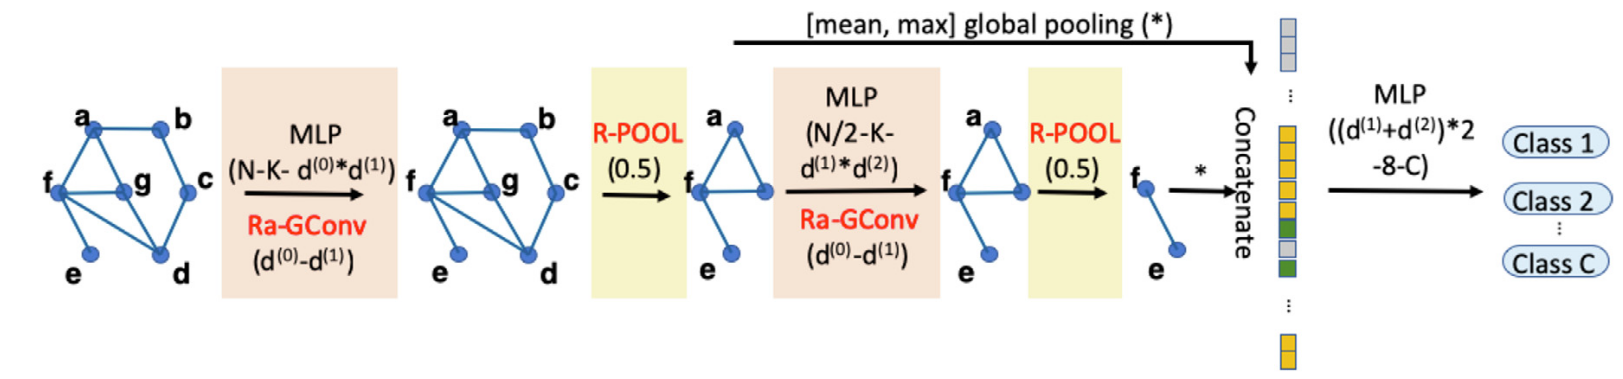
\includegraphics[width=1.0\linewidth]{figures/architecture.png}
	\caption{BrainGNN architecture}
	\cite{LI2021102233}
	\label{fig:architecture}
\end{figure}

\subsubsection{Graph convolutional layer}
\label{approach:Ba}

The node feature vectors of the whole graph are stored in the $H$ matrix. The goal of the convolutional layer is to learn new node feature vectors encoding the topological and semantical information of the graph.

The formula for the forward-pass update of the node feature vectors is defined by Schlichtkrull et al. \cite{10.1007/978-3-319-93417-4_38} as:

\begin{equation}\label{eq:conv_general}
\tilde{h}_i^{(l+1)} = \textrm{relu} \left( W_i^{(l)} h_i^{(l)} + \sum_{j \in \mathcal{N}^{(l)}(i)}^{} e_{ij}^{(l)} W_j^{(l)} h_j^{(l)} \right).
\end{equation}

The superscript $(l)$ denotes the layer and the subscript $i$ denotes the node.
The feature vector of node $i$ in layer $l+1$ is calculated by first multiplying the previous feature vector $h_i^{(l)}$ of node $i$ with the weights $W_i^{(l)}$. Then the feature vectors of all neighbors of node $i$ (neighbor = an edge exists between node $i$ and node $j$) are multiplied with the weights and summed. Up to now the formula is linear. To achieve nonlinearity, the result is passed through an activation function (in this case relu).

%TODO: term oben noch genauer erläutern? was die teilbereiche bedeuten?
%TODO: first iteration on orignal graph -> then on the new representation in following
%TODO: weight normalization

The general idea of the convolutional layer and the novelties of this work are illustrated in figure \ref{fig:convolution}.
\begin{figure}[ht]
	\centering
	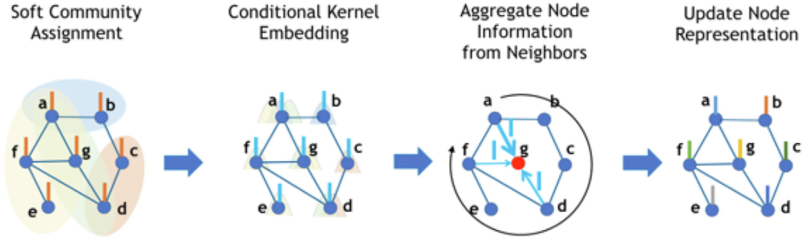
\includegraphics[width=1.0\linewidth]{figures/convolution.png}
	\caption{Graph convolutional layer operations}
	\cite{LI2021102233}
	\label{fig:convolution}
\end{figure}

The two proposed improvements in this work \cite{LI2021102233} for the graph convolutional layer are: 
\begin{enumerate}
	\item Learn different embedding weights for each ROI: \newline
	In eq \ref{eq:conv_general} the weights $W$ are the same for all nodes (ROIs). In this work individual weights are learned for each node. Finally, the vector $\textrm{vec}(W_i^{(l)})$ contains all learned node weights.
	
	The underlying assumption is, that the nodes at the same location but from different graphs are similar. Furthermore, a vector $r_i$ contains the regional information of node $i$ (e.g. the position in the graph). 
	The ordering of all nodes (ROIs) is consistent across different instances. To be able to learn new node feature vectors, which are independent of the ordering method, the regional information $r_i$ is stored as one-hot encoded vector.
	
	As described above the new node feature vector is calculated by ag\-gre\-ga\-ting the neighboring node feature vectors.
	For each node a computation graph of the neighbors is set up. The aggregation of node feature vectors is then done by a neural network with the parameters $\{\Theta_1^{(l)}, \Theta_2^{(l)}\}$ and the input $r_i$.
	
	\begin{equation}\label{eq:conv_1}
	\textrm{vec}(W_i^{(l)}) = f_{MLP}^{(l)}(r_i) = \Theta_2^{(l)} \textrm{relu}(\Theta_1^{(l)} r_i) + b^{(l)}.
	\end{equation}
	
	Eq \ref{eq:conv_1} can be reformulated to:
	\begin{equation}\label{eq:conv_2}
	\textrm{vec}(W_i^{(l)}) = \sum_{u=1}^{K^{(l)}} (\alpha_{iu}^{(l)})^+ \beta_u^{(l)} + b^{(l)}.
	\end{equation}
	
	The weights are decomposed into $\alpha$ (corresponds to $\Theta_1^{(l)}$) and $\beta$ (cor\-re\-sponds to $\Theta_2^{(l)}$). The matrix $\alpha$ contains information about the community membership of nodes. A basis vector for each community is stored in $\beta$.
	
	
	\item Include the edge weight: \newline
	The edge weights in the graph describe the coupling between two nodes. By multiplying node features with the edge weight the connection strength is taken into account.
\end{enumerate}


\subsubsection{Graph pooling layer}
\label{approach:Bb}

The goal of the graph pooling layer is the dimensionality reduction of the graph. Kaiser et al. \cite{doi:10.1073/pnas.1010412107} and Baker et al. \cite{10.1001/jamapsychiatry.2013.3469} have shown, that not all nodes are equally important for predicting neurological disorders. A dimensionality reduction is achieved by keeping the important nodes and removing the other nodes.
The pooling layer is implemented as proposed by Cangea et al. \cite{https://doi.org/10.48550/arxiv.1811.01287} and Gao and Ji \cite{pmlr-v97-gao19a}. For details, please refer to \cite{https://doi.org/10.48550/arxiv.1811.01287} and \cite{pmlr-v97-gao19a}.

The general idea of the pooling layer is illustrated in figure \ref{fig:pooling}. The input are the feature vectors from the convolutional layer. These vectors are then projected onto a learned pooling vector $w^{(l)}$. Based on the difference between the pooling vector and the node feature vectors, a score is calculated. Low scoring nodes are removed, and high scoring nodes are kept.

\begin{figure}[ht]
	\centering
	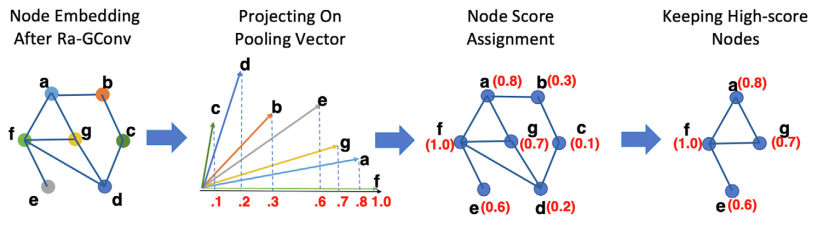
\includegraphics[width=1.0\linewidth]{figures/pooling.png}
	\caption{Graph pooling layer operations}
	\cite{LI2021102233}
	\label{fig:pooling}
\end{figure}

%TODO: Formeln hier aufführen oder weglassen?


%TODO: inwiefern noch auf den Readout layer eingehen?
%TODO: wirklich eigenes Kapitel oder droppen? MLP


\subsection{Training process: loss functions}
\label{approach:C}

As classification loss, the cross entropy loss is used:

\begin{equation}\label{eq:loss_ce}
	L_{ce} = -\frac{1}{M} \sum_{m=1}^{M} \sum_{c=1}^{C} y_{m,c} \log(\hat{y}_{m,c}).
\end{equation}

$M$ denotes the number of instances, $C$ the number of classes, $\hat{y}_{m, c}$ is the model prediction and $y_{m, c}$ is the ground truth label.

To enable interpretability further loss terms are used.
As introduced in section \ref{approach:Bb} a projection from the node representation onto a learned vector $w^{(l)} \in {\mathbb{R}}^{d^{(l)}}$ is used.
The scaling of this vector can vary, but the resulting scores remain the same. 
Consequently, it is not uniquely identifiable, which scores are produced by which learned vectors.
To overcome this issue, a unit loss enforces, that $w^{(l)}$ is a unit vector.

\begin{equation}\label{eq:loss_unit}
L_{unit}^{(l)} = (\| w^{(l)} \|_2 - 1)^2.
\end{equation}

A group-level consistency (GLC) loss is used to ensure, that in the pooling layer, the same nodes are selected across all input instances. This enables the detection of underlying patterns of a disease.
In deeper layers of the network, the graph structure changes. That is why this loss is only used after the first pooling layer, because here the graph structure is still the same as the input graph.

The GLC loss is defined as:

\begin{equation}\label{eq:loss_glc}
L_{GLC} = \sum_{c=1}^{C} \sum_{m,n \in \mathcal{I}_c}^{} \| \tilde{s}_m^{(1)} - \tilde{s}_n^{(1)} \|^2 = 2 \sum_{c=1}^{C} Tr((S_c^{(1)})^T L_c S_c^{(1)}).
\end{equation}

It calculates the pooling score similarity between two instances $m$ and $n$ ($\| \tilde{s}_m^{(1)} - \tilde{s}_n^{(1)} \|^2$). By taking the sum over all classes $C$ (first sum) and the sum over all instances $M$ in one batch (second sum), the pairwise pooling score similarities are calculated between all instances.
%By minimizing this GLC loss term, it is ensured, that the scores of the instances are similar and therefore the selection of nodes for removing or keeping is similar.
%If the scores of two instances are similar, the GLC loss is low.
The way how this is calculated is expressed on the right hand side of the equation. For details about this, please refer to \cite{LI2021102233}.

The TopK pooling loss makes sure, that the nodes which are removed have a significantly different score compared to the nodes which are not removed. 
First of all, the scores are passed through a sigmoid layer. After this, the score values are in the range between 0 and 1. These scores are then sorted in descending order for all $M$ instances. Finally, a constraint is applied to the ordering for all $M$ instances, which leads to a more dispersed distribution. 
Mathematically, it is formulated as binary cross-entropy:

\begin{equation}\label{eq:loss_tpk}
L_{TPK}^{(l)} = - \frac{1}{M} \sum_{m=1}^{M} \frac{1}{N^{(l)}} \left(\sum_{i=1}^{k} \log(\hat{s}_{m, i}^{(l)}) + \sum_{i=1}^{N^{(l)}-k} \log (1- \hat{s}_{m, i+k}^{(l)})\right).
\end{equation}

All presented loss functions above are part of the final loss function (with $\lambda_1$ and $\lambda_2$ as hyperparameters):

\begin{equation}\label{eq:loss_total}
L_{total} = L_{ce} + \sum_{l=1}^{L} L_{unit}^{(l)} + \lambda_1 \sum_{l=1}^{L} L_{TPK}^{(l)} + \lambda_2 L_{GLC}.
\end{equation}

\section{Experiments and results} \label{experimental_setup}

%\subsection{Evaluation datasets}
%\label{experimental_setup:A}

The proposed BrainGNN is evaluated on two datasets. On the one hand the Biopoint Autism Study Dataset (Biopoint) \cite{Venkataraman2016BayesianCD} is used. It deals with a binary prediction task, whether a patient has autism or not. On the other hand the Human Connectome Project (HCP) 900 Subject Release dataset \cite{VANESSEN201362} is used. The task is a multi class classification, to distinguish between different tasks (e.g. motorical task, language task, gambling). For details about the datasets, please refer to  \cite{Venkataraman2016BayesianCD} and \cite{VANESSEN201362}.

%\subsection{Prediction results}
%\label{experimental_setup:B}

Table \ref{fig:prediction_results} shows the prediction results of BrainGNN in comparison to other approaches. For both datasets, BrainGNN outperforms all other approaches.

\begin{figure}[ht]
	\centering
	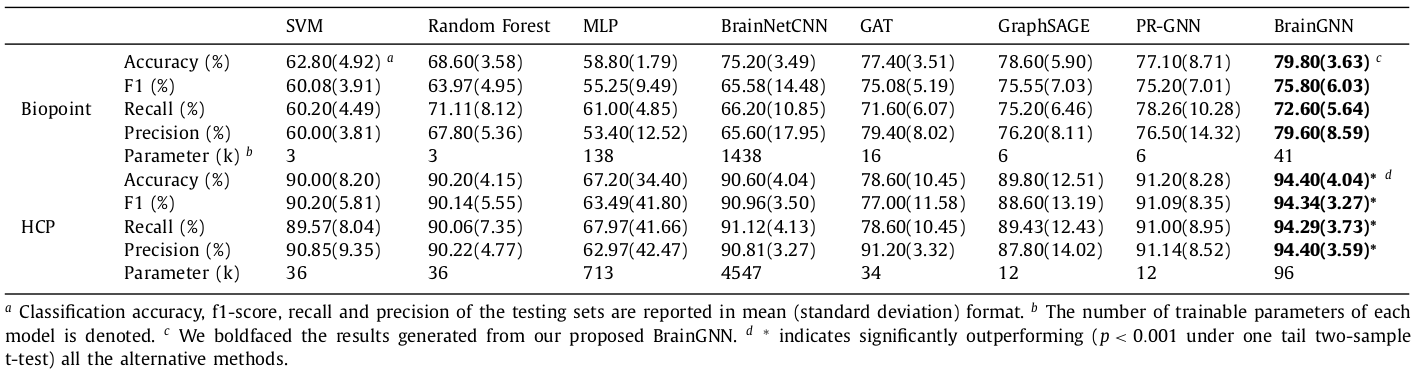
\includegraphics[width=1.0\linewidth]{figures/predictionResults.png}
	\caption{Prediction results of BrainGNN compared to other baseline approaches}
	\cite{LI2021102233}
	\label{fig:prediction_results}
\end{figure}

%\subsection{Interpretation results}
%\label{experimental_setup:C}

Besides the classification, the interpretation of the results is also possible.
On the one hand, the detection of biomarkers is possible. For both datasets the detected biomarkers are validated by literature. 
On the other hand the detected brain community patterns can be interpreted.
For a detailed description of the interpretation process, please refer to \cite{LI2021102233}.

\section{Discussion} \label{analysis}

%Limitations and future work
The preprocessing steps from Li et al. \cite{LI2021102233} (all steps from fMRI imaging up to the construction of the functional graph) are one possible way, how this could be done. 
In their work, they have used one brain parcellation atlas. For future work the usage of different brain parcellation atlases and the comparison of the results would be interesting. Furthermore, the authors regard an end-to-end training procedure, which extracts relevant features automatically from the fMRI imaging as part of the trained model as a challenging but promising direction for future work.

The BrainGNN model can be further improved through a more detailed hyperparameter tuning. Moreover, more quantitative and theoretical studies are needed to fully understand the proposed graph convolutional layer.

The results of BrainGNN can be improved by evaluating failure prediction cases to answer the question, if there are specific patterns, where the model always fails. 
Finally, the whole proposed model could be tested on other datasets and problems.

The work from Li et al. \cite{LI2021102233} was used in subsequent work as baseline for comparing results and as starting point for model architecture improvements.
Lin et al. \cite{LIN2022102430} use the proposed BrainGNN from Li et al. \cite{LI2021102233} as a baseline for comparing their 3D-CNN architecture. As evaluation dataset they used a schizophrenia dataset. 
Gao et al. \cite{gaoSexDifferencesCerebellum2022} built their work upon Li et al. \cite{LI2021102233} and apply the GNN to sex prediction and interpretation of the differences related to sex.
Wen et al. \cite{WEN2022105239} propose an optimized GNN architecture and use the BrainGNN from Li et al. \cite{LI2021102233} among other approaches as baseline. 

\section{Conclusion} \label{conclusion}

The work by Li et al. \cite{LI2021102233} proposes a novel Brain Graph Neural Network for fMRI analysis. The two main innovations are the improved graph con\-vo\-lu\-tio\-nal layer and the inbuilt interpretability through various loss terms as part of the graph pooling layer.

The result of Li et al. \cite{LI2021102233} is a BrainGNN model, which outperforms all other approaches for both prediction tasks. Furthermore the detection of group-level and individual-level biomarkers is possible. Moreover it is possible to detect brain communities.

Through this work the understanding of neurological diseases can be improved, which is essential for the development of personalized treatments in the area of precision medicine.

%\clearpage
%\pagenumbering{Roman}
%\appendix
%\section{Appendix}

\subsection{Experimental details}
\label{ch:app-A}


%%%%%%%%%%%%%%%%%%%%%%%%%%%%%%%%%%%%%%%%%%%%%%%%%%%%%%%%%%%%

%\newpage
\section{References}
\printbibliography[heading=none]

\end{document}
